% Options for packages loaded elsewhere
\PassOptionsToPackage{unicode}{hyperref}
\PassOptionsToPackage{hyphens}{url}
%
\documentclass[
]{article}
\title{bayesruleswork\_ch2.1.5}
\author{cl}
\date{27/01/2022}

\usepackage{amsmath,amssymb}
\usepackage{lmodern}
\usepackage{iftex}
\ifPDFTeX
  \usepackage[T1]{fontenc}
  \usepackage[utf8]{inputenc}
  \usepackage{textcomp} % provide euro and other symbols
\else % if luatex or xetex
  \usepackage{unicode-math}
  \defaultfontfeatures{Scale=MatchLowercase}
  \defaultfontfeatures[\rmfamily]{Ligatures=TeX,Scale=1}
\fi
% Use upquote if available, for straight quotes in verbatim environments
\IfFileExists{upquote.sty}{\usepackage{upquote}}{}
\IfFileExists{microtype.sty}{% use microtype if available
  \usepackage[]{microtype}
  \UseMicrotypeSet[protrusion]{basicmath} % disable protrusion for tt fonts
}{}
\makeatletter
\@ifundefined{KOMAClassName}{% if non-KOMA class
  \IfFileExists{parskip.sty}{%
    \usepackage{parskip}
  }{% else
    \setlength{\parindent}{0pt}
    \setlength{\parskip}{6pt plus 2pt minus 1pt}}
}{% if KOMA class
  \KOMAoptions{parskip=half}}
\makeatother
\usepackage{xcolor}
\IfFileExists{xurl.sty}{\usepackage{xurl}}{} % add URL line breaks if available
\IfFileExists{bookmark.sty}{\usepackage{bookmark}}{\usepackage{hyperref}}
\hypersetup{
  pdftitle={bayesruleswork\_ch2.1.5},
  pdfauthor={cl},
  hidelinks,
  pdfcreator={LaTeX via pandoc}}
\urlstyle{same} % disable monospaced font for URLs
\usepackage[margin=1in]{geometry}
\usepackage{color}
\usepackage{fancyvrb}
\newcommand{\VerbBar}{|}
\newcommand{\VERB}{\Verb[commandchars=\\\{\}]}
\DefineVerbatimEnvironment{Highlighting}{Verbatim}{commandchars=\\\{\}}
% Add ',fontsize=\small' for more characters per line
\usepackage{framed}
\definecolor{shadecolor}{RGB}{248,248,248}
\newenvironment{Shaded}{\begin{snugshade}}{\end{snugshade}}
\newcommand{\AlertTok}[1]{\textcolor[rgb]{0.94,0.16,0.16}{#1}}
\newcommand{\AnnotationTok}[1]{\textcolor[rgb]{0.56,0.35,0.01}{\textbf{\textit{#1}}}}
\newcommand{\AttributeTok}[1]{\textcolor[rgb]{0.77,0.63,0.00}{#1}}
\newcommand{\BaseNTok}[1]{\textcolor[rgb]{0.00,0.00,0.81}{#1}}
\newcommand{\BuiltInTok}[1]{#1}
\newcommand{\CharTok}[1]{\textcolor[rgb]{0.31,0.60,0.02}{#1}}
\newcommand{\CommentTok}[1]{\textcolor[rgb]{0.56,0.35,0.01}{\textit{#1}}}
\newcommand{\CommentVarTok}[1]{\textcolor[rgb]{0.56,0.35,0.01}{\textbf{\textit{#1}}}}
\newcommand{\ConstantTok}[1]{\textcolor[rgb]{0.00,0.00,0.00}{#1}}
\newcommand{\ControlFlowTok}[1]{\textcolor[rgb]{0.13,0.29,0.53}{\textbf{#1}}}
\newcommand{\DataTypeTok}[1]{\textcolor[rgb]{0.13,0.29,0.53}{#1}}
\newcommand{\DecValTok}[1]{\textcolor[rgb]{0.00,0.00,0.81}{#1}}
\newcommand{\DocumentationTok}[1]{\textcolor[rgb]{0.56,0.35,0.01}{\textbf{\textit{#1}}}}
\newcommand{\ErrorTok}[1]{\textcolor[rgb]{0.64,0.00,0.00}{\textbf{#1}}}
\newcommand{\ExtensionTok}[1]{#1}
\newcommand{\FloatTok}[1]{\textcolor[rgb]{0.00,0.00,0.81}{#1}}
\newcommand{\FunctionTok}[1]{\textcolor[rgb]{0.00,0.00,0.00}{#1}}
\newcommand{\ImportTok}[1]{#1}
\newcommand{\InformationTok}[1]{\textcolor[rgb]{0.56,0.35,0.01}{\textbf{\textit{#1}}}}
\newcommand{\KeywordTok}[1]{\textcolor[rgb]{0.13,0.29,0.53}{\textbf{#1}}}
\newcommand{\NormalTok}[1]{#1}
\newcommand{\OperatorTok}[1]{\textcolor[rgb]{0.81,0.36,0.00}{\textbf{#1}}}
\newcommand{\OtherTok}[1]{\textcolor[rgb]{0.56,0.35,0.01}{#1}}
\newcommand{\PreprocessorTok}[1]{\textcolor[rgb]{0.56,0.35,0.01}{\textit{#1}}}
\newcommand{\RegionMarkerTok}[1]{#1}
\newcommand{\SpecialCharTok}[1]{\textcolor[rgb]{0.00,0.00,0.00}{#1}}
\newcommand{\SpecialStringTok}[1]{\textcolor[rgb]{0.31,0.60,0.02}{#1}}
\newcommand{\StringTok}[1]{\textcolor[rgb]{0.31,0.60,0.02}{#1}}
\newcommand{\VariableTok}[1]{\textcolor[rgb]{0.00,0.00,0.00}{#1}}
\newcommand{\VerbatimStringTok}[1]{\textcolor[rgb]{0.31,0.60,0.02}{#1}}
\newcommand{\WarningTok}[1]{\textcolor[rgb]{0.56,0.35,0.01}{\textbf{\textit{#1}}}}
\usepackage{graphicx}
\makeatletter
\def\maxwidth{\ifdim\Gin@nat@width>\linewidth\linewidth\else\Gin@nat@width\fi}
\def\maxheight{\ifdim\Gin@nat@height>\textheight\textheight\else\Gin@nat@height\fi}
\makeatother
% Scale images if necessary, so that they will not overflow the page
% margins by default, and it is still possible to overwrite the defaults
% using explicit options in \includegraphics[width, height, ...]{}
\setkeys{Gin}{width=\maxwidth,height=\maxheight,keepaspectratio}
% Set default figure placement to htbp
\makeatletter
\def\fps@figure{htbp}
\makeatother
\setlength{\emergencystretch}{3em} % prevent overfull lines
\providecommand{\tightlist}{%
  \setlength{\itemsep}{0pt}\setlength{\parskip}{0pt}}
\setcounter{secnumdepth}{-\maxdimen} % remove section numbering
\ifLuaTeX
  \usepackage{selnolig}  % disable illegal ligatures
\fi

\begin{document}
\maketitle

\hypertarget{bayes-rules-textbook-work-ch.2.1.5}{%
\subsection{Bayes rules textbook work
Ch.2.1.5}\label{bayes-rules-textbook-work-ch.2.1.5}}

\begin{Shaded}
\begin{Highlighting}[]
\FunctionTok{library}\NormalTok{(bayesrules)}
\FunctionTok{library}\NormalTok{(tidyverse)}
\end{Highlighting}
\end{Shaded}

\begin{verbatim}
## -- Attaching packages --------------------------------------- tidyverse 1.3.1 --
\end{verbatim}

\begin{verbatim}
## v ggplot2 3.3.5     v purrr   0.3.4
## v tibble  3.1.4     v dplyr   1.0.7
## v tidyr   1.1.4     v stringr 1.4.0
## v readr   2.1.1     v forcats 0.5.1
\end{verbatim}

\begin{verbatim}
## -- Conflicts ------------------------------------------ tidyverse_conflicts() --
## x dplyr::filter() masks stats::filter()
## x dplyr::lag()    masks stats::lag()
\end{verbatim}

\begin{Shaded}
\begin{Highlighting}[]
\FunctionTok{library}\NormalTok{(janitor)}
\end{Highlighting}
\end{Shaded}

\begin{verbatim}
## 
## Attaching package: 'janitor'
\end{verbatim}

\begin{verbatim}
## The following objects are masked from 'package:stats':
## 
##     chisq.test, fisher.test
\end{verbatim}

\begin{Shaded}
\begin{Highlighting}[]
\CommentTok{\# Define possible articles}
\NormalTok{article }\OtherTok{\textless{}{-}} \FunctionTok{data.frame}\NormalTok{(}\AttributeTok{type =} \FunctionTok{c}\NormalTok{(}\StringTok{"real"}\NormalTok{, }\StringTok{"fake"}\NormalTok{))}

\CommentTok{\# Define the prior model}
\NormalTok{prior }\OtherTok{\textless{}{-}} \FunctionTok{c}\NormalTok{(}\FloatTok{0.6}\NormalTok{, }\FloatTok{0.4}\NormalTok{)}
\CommentTok{\# Simulate 3 articles}
\FunctionTok{sample\_n}\NormalTok{(article, }\AttributeTok{size =} \DecValTok{3}\NormalTok{, }\AttributeTok{weight =}\NormalTok{ prior, }\AttributeTok{replace =} \ConstantTok{TRUE}\NormalTok{)}
\end{Highlighting}
\end{Shaded}

\begin{verbatim}
##   type
## 1 real
## 2 real
## 3 real
\end{verbatim}

\begin{Shaded}
\begin{Highlighting}[]
\CommentTok{\# Set the seed. Simulate 3 articles.}
\FunctionTok{set.seed}\NormalTok{(}\DecValTok{84735}\NormalTok{)}
\FunctionTok{sample\_n}\NormalTok{(article, }\AttributeTok{size =} \DecValTok{3}\NormalTok{, }\AttributeTok{weight =}\NormalTok{ prior, }\AttributeTok{replace =} \ConstantTok{TRUE}\NormalTok{)}
\end{Highlighting}
\end{Shaded}

\begin{verbatim}
##   type
## 1 fake
## 2 fake
## 3 real
\end{verbatim}

\begin{Shaded}
\begin{Highlighting}[]
\CommentTok{\# Simulate 10000 articles. }
\FunctionTok{set.seed}\NormalTok{(}\DecValTok{84735}\NormalTok{)}
\NormalTok{article\_sim }\OtherTok{\textless{}{-}} \FunctionTok{sample\_n}\NormalTok{(article, }\AttributeTok{size =} \DecValTok{10000}\NormalTok{, }\AttributeTok{weight =}\NormalTok{ prior, }\AttributeTok{replace =} \ConstantTok{TRUE}\NormalTok{)}
\FunctionTok{ggplot}\NormalTok{(article\_sim, }\FunctionTok{aes}\NormalTok{(}\AttributeTok{x =}\NormalTok{ type)) }\SpecialCharTok{+} \FunctionTok{geom\_bar}\NormalTok{()}
\end{Highlighting}
\end{Shaded}

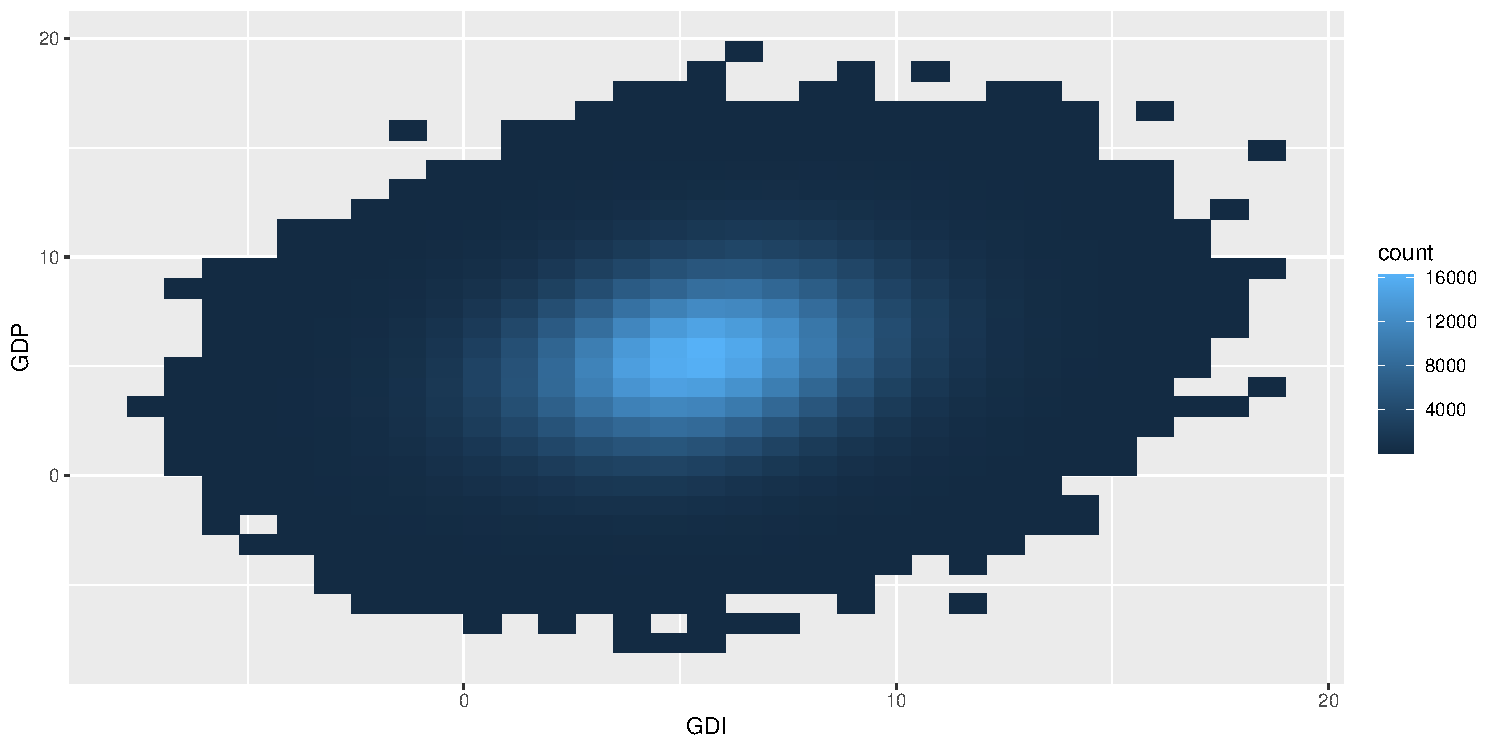
\includegraphics{testsave_files/figure-latex/unnamed-chunk-2-1.pdf}

\begin{Shaded}
\begin{Highlighting}[]
\CommentTok{\#article\_sim \%\textgreater{}\% }
\CommentTok{\#+     tabyl(type) \%\textgreater{}\% }
\CommentTok{\#+     adorn\_totals("row")}

\CommentTok{\#article\_sim \textless{}{-} article\_sim \%\textgreater{}\% }
\CommentTok{\#+     mutate(data\_model = case\_when(type == "fake" \textasciitilde{} 0.2667,}
\CommentTok{\#+                                   type == "real" \textasciitilde{} 0.0222))}
\CommentTok{\#\textgreater{} }
\CommentTok{\#glimpse(article\_sim)}
\end{Highlighting}
\end{Shaded}

\begin{Shaded}
\begin{Highlighting}[]
\CommentTok{\# Define whether there are exclamation points}
\CommentTok{\#data \textless{}{-} c("no", "yes")}
 
\CommentTok{\# Simulate exclamation point usage }
\CommentTok{\#set.seed(3)}
\CommentTok{\#article\_sim \textless{}{-} article\_sim \%\textgreater{}\%}
\CommentTok{\#+     group\_by(1:n()) \%\textgreater{}\% }
\CommentTok{\#+     mutate(usage = sample(data, size = 1, }
\CommentTok{\#+                           prob = c(1 {-} data\_model, data\_model)))}
\CommentTok{\#article\_sim \%\textgreater{}\% }
\CommentTok{\#+     tabyl(usage, type) \%\textgreater{}\% }
\CommentTok{\#+     adorn\_totals(c("col","row"))}
\end{Highlighting}
\end{Shaded}

\begin{Shaded}
\begin{Highlighting}[]
\CommentTok{\#\textgreater{} ggplot(article\_sim, aes(x = type, fill = usage)) + }
\CommentTok{\#+     geom\_bar(position = "fill")}
\CommentTok{\#\textgreater{} ggplot(article\_sim, aes(x = type)) + }
\CommentTok{\#+     geom\_bar()}
\end{Highlighting}
\end{Shaded}

\begin{Shaded}
\begin{Highlighting}[]
\CommentTok{\#\textgreater{} article\_sim \%\textgreater{}\% }
\CommentTok{\#+     filter(usage == "yes") \%\textgreater{}\% }
\CommentTok{\#+     tabyl(type) \%\textgreater{}\% }
\CommentTok{\#+     adorn\_totals("row")}
\end{Highlighting}
\end{Shaded}

insert some comments here to try out r-markdown

\begin{Shaded}
\begin{Highlighting}[]
\CommentTok{\#\textgreater{} ggplot(article\_sim, aes(x = type)) + }
\CommentTok{\#+     geom\_bar() + }
\CommentTok{\#+     facet\_wrap(\textasciitilde{} usage)}
\end{Highlighting}
\end{Shaded}


\end{document}
